\documentclass{standalone}

\usepackage{siunitx}
\usepackage{pgfplots}
\usepackage{pgfplotstable}

\begin{document}

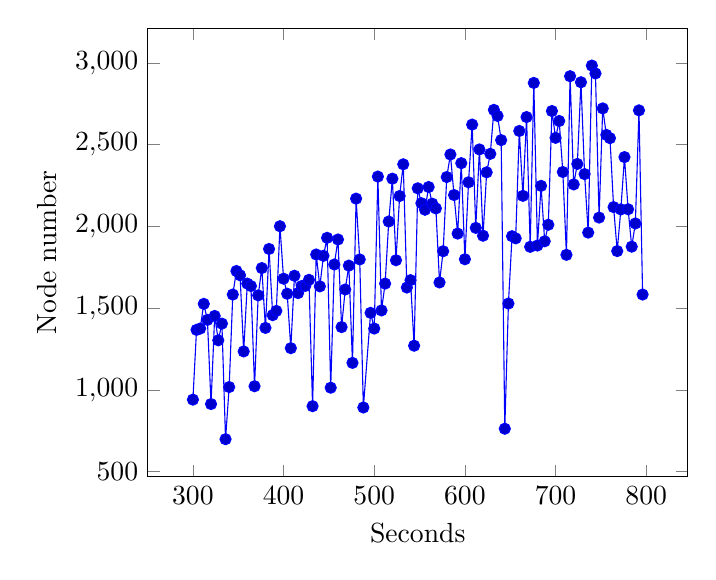
\begin{tikzpicture}
	\begin{axis}[
		xlabel=Seconds,
		ylabel={Node number}
	]
	\addplot coordinates{
		(300,940)
		(304,1367)
		(308,1375)
		(312,1526)
		(316,1428)
		(320,913)
		(324,1452)
		(328,1303)
		(332,1405)
		(336,698)
		(340,1017)
		(344,1583)
		(348,1727)
		(352,1701)
		(356,1235)
		(360,1650)
		(364,1635)
		(368,1022)
		(372,1578)
		(376,1745)
		(380,1379)
		(384,1862)
		(388,1457)
		(392,1483)
		(396,2001)
		(400,1680)
		(404,1588)
		(408,1255)
		(412,1698)
		(416,1592)
		(420,1635)
		(424,1636)
		(428,1673)
		(432,900)
		(436,1828)
		(440,1633)
		(444,1820)
		(448,1930)
		(452,1013)
		(456,1767)
		(460,1920)
		(464,1384)
		(468,1614)
		(472,1760)
		(476,1165)
		(480,2170)
		(484,1798)
		(488,892)
		(496,1471)
		(500,1375)
		(504,2305)
		(508,1486)
		(512,1650)
		(516,2030)
		(520,2292)
		(524,1793)
		(528,2186)
		(532,2380)
		(536,1626)
		(540,1671)
		(544,1270)
		(548,2233)
		(552,2142)
		(556,2102)
		(560,2241)
		(564,2139)
		(568,2110)
		(572,1657)
		(576,1848)
		(580,2302)
		(584,2440)
		(588,2192)
		(592,1956)
		(596,2387)
		(600,1799)
		(604,2270)
		(608,2623)
		(612,1991)
		(616,2471)
		(620,1943)
		(624,2331)
		(628,2444)
		(632,2713)
		(636,2676)
		(640,2528)
		(644,762)
		(648,1528)
		(652,1940)
		(656,1927)
		(660,2584)
		(664,2187)
		(668,2669)
		(672,1875)
		(676,2878)
		(680,1883)
		(684,2248)
		(688,1909)
		(692,2010)
		(696,2706)
		(700,2542)
		(704,2645)
		(708,2333)
		(712,1826)
		(716,2919)
		(720,2257)
		(724,2382)
		(728,2882)
		(732,2320)
		(736,1962)
		(740,2984)
		(744,2936)
		(748,2054)
		(752,2722)
		(756,2560)
		(760,2540)
		(764,2118)
		(768,1849)
		(772,2104)
		(776,2424)
		(780,2105)
		(784,1876)
		(788,2018)
		(792,2710)
		(796,1583)
	};
	\end{axis}
\end{tikzpicture}

\end{document}
